% Lines starting with a percent sign (%) are comments. LaTeX will 
% not process those lines. Similarly, everything after a percent 
% sign in a line is considered a comment. To produce a percent sign
% in the output, write \% (backslash followed by the percent sign). 
% ==================================================================
% Usage instructions:
% ------------------------------------------------------------------
% The file is heavily commented so that you know what the various
% commands do. Feel free to remove any comments you don't need from
% your own copy. When redistributing the example thesis file, please
% retain all the comments for the benefit of other thesis writers! 
% ==================================================================
% Compilation instructions: 
% ------------------------------------------------------------------
% Use pdflatex to compile! Input images are expected as PDF files.
% Example compilation:
% ------------------------------------------------------------------
% > pdflatex thesis-example.tex
% > bibtex thesis-example
% > pdflatex thesis-example.tex
% > pdflatex thesis-example.tex
% ------------------------------------------------------------------
% You need to run pdflatex multiple times so that all the cross-references
% are fixed. pdflatex will tell you if you need to re-run it (a warning
% will be issued)  
% ------------------------------------------------------------------
% Compilation has been tested to work in ukk.cs.hut.fi and kosh.hut.fi
% - if you have problems of missing .sty -files, then the local LaTeX
% environment does not have all the required packages installed.
% For example, when compiling in vipunen.hut.fi, you get an error that
% tikz.sty is missing - in this case you must either compile somewhere
% else, or you cannot use TikZ graphics in your thesis and must therefore
% remove or comment out the tikz package and all the tikz definitions. 
% ------------------------------------------------------------------

% General information
% ==================================================================
% Package documentation:
% 
% The comments often refer to package documentation. (Almost) all LaTeX
% packages have documentation accompanying them, so you can read the
% package documentation for further information. When a package 'xxx' is
% installed to your local LaTeX environment (the document compiles
% when you have \usepackage{xxx} and LaTeX does not complain), you can 
% find the documentation somewhere in the local LaTeX texmf directory
% hierarchy. In ukk.cs.hut.fi, this is /usr/texlive/2008/texmf-dist,
% and the documentation for the titlesec package (for example) can be 
% found at /usr/texlive/2008/texmf-dist/doc/latex/titlesec/titlesec.pdf.
% Most often the documentation is located as a PDF file in 
% /usr/texlive/2008/texmf-dist/doc/latex/xxx, where xxx is the package name; 
% however, documentation for TikZ is in
% /usr/texlive/2008/texmf-dist/doc/latex/generic/pgf/pgfmanual.pdf
% (this is because TikZ is a front-end for PGF, which is meant to be a 
% generic portable graphics format for LaTeX).
% You can try to look for the package manual using the ``find'' shell
% command in Linux machines; the find databases are up-to-date at least
% in ukk.cs.hut.fi. Just type ``find xxx'', where xxx is the package
% name, and you should find a documentation file.
% Note that in some packages, the documentation is in the DVI file
% format. In this case, you can copy the DVI file to your home directory,
% and convert it to PDF with the dvipdfm command (or you can read the
% DVI file directly with a DVI viewer).
% 
% If you can't find the documentation for a package, just try Googling
% for ``latex packagename''; most often you can get a direct link to the
% package manual in PDF format.
% ------------------------------------------------------------------


% Document class for the thesis is report
% ------------------------------------------------------------------
% You can change this but do so at your own risk - it may break other things.
% Note that the option pdftext is used for pdflatex; there is no
% pdflatex option. 
% ------------------------------------------------------------------
\documentclass[12pt,a4paper,oneside,pdftex]{report}

% The input files (tex files) are encoded with the latin-1 encoding 
% (ISO-8859-1 works). Change the latin1-option if you use UTF8 
% (at some point LaTeX did not work with UTF8, but I'm not sure
% what the current situation is) 
\usepackage[utf8]{inputenc}
% OT1 font encoding seems to work better than T1. Check the rendered
% PDF file to see if the fonts are encoded properly as vectors (instead
% of rendered bitmaps). You can do this by zooming very close to any letter 
% - if the letter is shown pixelated, you should change this setting 
% (try commenting out the entire line, for example).  
\usepackage[OT1]{fontenc}
% The babel package provides hyphenating instructions for LaTeX. Give
% the languages you wish to use in your thesis as options to the babel
% package (as shown below). You can remove any language you are not
% going to use.
% Examples of valid language codes: english (or USenglish), british, 
% finnish, swedish; and so on.
\usepackage[finnish,english]{babel}


% Font selection
% ------------------------------------------------------------------
% The default LaTeX font is a very good font for rendering your 
% thesis. It is a very professional font, which will always be 
% accepted. 
% If you, however, wish to spicen up your thesis, you can try out
% these font variants by uncommenting one of the following lines
% (or by finding another font package). The fonts shown here are 
% all fonts that you could use in your thesis (not too silly). 
% Changing the font causes the layouts to shift a bit; you many
% need to manually adjust some layouts. Check the warning messages
% LaTeX gives you.
% ------------------------------------------------------------------
% To find another font, check out the font catalogue from
% http://www.tug.dk/FontCatalogue/mathfonts.html
% This link points to the list of fonts that support maths, but
% that's a fairly important point for master's theses.
% ------------------------------------------------------------------
% <rant>
% Remember, there is no excuse to use Comic Sans, ever, in any
% situation! (Well, maybe in speech bubbles in comics, but there 
% are better options for those too)
% </rant>

% \usepackage{palatino}
% \usepackage{tgpagella}



% Optional packages
% ------------------------------------------------------------------
% Select those packages that you need for your thesis. You may delete
% or comment the rest.

% Natbib allows you to select the format of the bibliography references.
% The first example uses numbered citations: 
\usepackage[square]{natbib}
\usepackage[nottoc,notlot,notlof]{tocbibind}
% The second example uses author-year citations.
% If you use author-year citations, change the bibliography style (below); 
% acm style does not work with author-year citations.
% Also, you should use \citet (cite in text) when you wish to refer
% to the author directly (\citet{blaablaa} said blaa blaa), and 
% \citep when you wish to refer similarly than with numbered citations
% (It has been said that blaa blaa~\citep{blaablaa}).
% \usepackage[square]{natbib}

% The alltt package provides an all-teletype environment that acts
% like verbatim but you can use LaTeX commands in it. Uncomment if 
% you want to use this environment. 
% \usepackage{alltt}

% The eurosym package provides a euro symbol. Use with \euro{}
\usepackage{eurosym} 

% Verbatim provides a standard teletype environment that renderes
% the text exactly as written in the tex file. Useful for code
% snippets (although you can also use the listings package to get
% automatic code formatting). 
\usepackage{verbatim}

% The listing package provides automatic code formatting utilities
% so that you can copy-paste code examples and have them rendered
% nicely. See the package documentation for details.
% \usepackage{listings}

% The fancuvrb package provides fancier verbatim environments 
% (you can, for example, put borders around the verbatim text area
% and so on). See package for details.
% \usepackage{fancyvrb}

% Supertabular provides a tabular environment that can span multiple 
% pages. 
%\usepackage{supertabular}
% Longtable provides a tabular environment that can span multiple 
% pages. This is used in the example acronyms file. 
\usepackage{longtable}

% The fancyhdr package allows you to set your the page headers 
% manually, and allows you to add separator lines and so on. 
% Check the package documentation. 
% \usepackage{fancyhdr}

% Subfigure package allows you to use subfigures (i.e. many subfigures
% within one figure environment). These can have different labels and
% they are numbered automatically. Check the package documentation. 
\usepackage{subfigure}

% The titlesec package can be used to alter the look of the titles 
% of sections, chapters, and so on. This example uses the ``medium'' 
% package option which sets the titles to a medium size, making them
% a bit smaller than what is the default. You can fine-tune the 
% title fonts and sizes by using the package options. See the package
% documentation.
\usepackage[medium]{titlesec}

% The TikZ package allows you to create professional technical figures.
% The learning curve is quite steep, but it is definitely worth it if 
% you wish to have really good-looking technical figures. 
\usepackage{tikz}
% You also need to specify which TikZ libraries you use
\usetikzlibrary{positioning}
\usetikzlibrary{calc}
\usetikzlibrary{arrows}
\usetikzlibrary{decorations.pathmorphing,decorations.markings}
\usetikzlibrary{shapes}
\usetikzlibrary{patterns}


% The aalto-thesis package provides typesetting instructions for the
% standard master's thesis parts (abstracts, front page, and so on)
% Load this package second-to-last, just before the hyperref package.
% Options that you can use: 
%   mydraft - renders the thesis in draft mode. 
%             Do not use for the final version. 
%   doublenumbering - [optional] number the first pages of the thesis
%                     with roman numerals (i, ii, iii, ...); and start
%                     arabic numbering (1, 2, 3, ...) only on the 
%                     first page of the first chapter
%   twoinstructors  - changes the title of instructors to plural form
%   twosupervisors  - changes the title of supervisors to plural form
\usepackage[mydraft,doublenumbering]{aalto-thesis}
%\usepackage[mydraft,doublenumbering]{aalto-thesis}
%\usepackage{aalto-thesis}

\usepackage{todo}
\usepackage{gensymb}
\usepackage{graphicx}


% Hyperref
% ------------------------------------------------------------------
% Hyperref creates links from URLs, for references, and creates a
% TOC in the PDF file.
% This package must be the last one you include, because it has
% compatibility issues with many other packages and it fixes
% those issues when it is loaded.   
\RequirePackage[pdftex]{hyperref}
% Setup hyperref so that links are clickable but do not look 
% different
\hypersetup{colorlinks=false,raiselinks=false,breaklinks=true}
\hypersetup{pdfborder={0 0 0}}
\hypersetup{bookmarksnumbered=true}
% The following line suggests the PDF reader that it should show the 
% first level of bookmarks opened in the hierarchical bookmark view. 
\hypersetup{bookmarksopen=true,bookmarksopenlevel=1}
% Hyperref can also set up the PDF metadata fields. These are
% set a bit later on, after the thesis setup.   


% Thesis setup
% ==================================================================
% Change these to fit your own thesis.
% \COMMAND always refers to the English version;
% \FCOMMAND refers to the Finnish version; and
% \SCOMMAND refers to the Swedish version.
% You may comment/remove those language variants that you do not use
% (but then you must not include the abstracts for that language)
% ------------------------------------------------------------------
% If you do not find the command for a text that is shown in the cover page or
% in the abstract texts, check the aalto-thesis.sty file and locate the text
% from there. 
% All the texts are configured in language-specific blocks (lots of commands
% that look like this: \renewcommand{\ATCITY}{Espoo}.
% You can just fix the texts there. Just remember to check all the language
% variants you use (they are all there in the same place). 
% ------------------------------------------------------------------
\newcommand{\TITLE}{An open and general CNC and machine vision based architecture for payment terminal acceptance test automation}
\newcommand{\FTITLE}{Ohjelmistoprosessit mänteille}
\newcommand{\STITLE}{Den stora stygga vargen}
\newcommand{\DATE}{May 13, 2016}
\newcommand{\FDATE}{13. toukokuuta 2016}
\newcommand{\SDATE}{Den 18 Juni 2011}

% Supervisors and instructors
% ------------------------------------------------------------------
% If you have two supervisors, write both names here, separate them with a 
% double-backslash (see below for an example)
% Also remember to add the package option ``twosupervisors'' or
% ``twoinstructors'' to the aalto-thesis package so that the titles are in
% plural.
% Example of one supervisor:
%\newcommand{\SUPERVISOR}{Professor Antti Ylä-Jääski}
%\newcommand{\FSUPERVISOR}{Professori Antti Ylä-Jääski}
%\newcommand{\SSUPERVISOR}{Professor Antti Ylä-Jääski}
% Example of twosupervisors:
\newcommand{\SUPERVISOR}{D.Sc. Seppo Sierla}
\newcommand{\FSUPERVISOR}{D.Sc. Seppo Sierla}
\newcommand{\SSUPERVISOR}{Professor Antti Ylä-Jääski}

% If you have only one instructor, just write one name here
\newcommand{\INSTRUCTOR}{Tatu Kairi M.Sc.}
\newcommand{\FINSTRUCTOR}{Filosofian maisteri Tatu Kairi}
\newcommand{\SINSTRUCTOR}{Diplomingenjör Olli Ohjaaja}
% If you have two instructors, separate them with \\ to create linefeeds
% \newcommand{\INSTRUCTOR}{Olli Ohjaaja M.Sc. (Tech.)\\
%  Elli Opas M.Sc. (Tech)}
%\newcommand{\FINSTRUCTOR}{Diplomi-insinööri Olli Ohjaaja\\
%  Diplomi-insinööri Elli Opas}
%\newcommand{\SINSTRUCTOR}{Diplomingenjör Olli Ohjaaja\\
%  Diplomingenjör Elli Opas}

% If you have two supervisors, it is common to write the schools
% of the supervisors in the cover page. If the following command is defined,
% then the supervisor names shown here are printed in the cover page. Otherwise,
% the supervisor names defined above are used.
\newcommand{\COVERSUPERVISOR}{D.Sc. Seppo Sierla, Aalto University}

% The same option is for the instructors, if you have multiple instructors.
% \newcommand{\COVERINSTRUCTOR}{Olli Ohjaaja M.Sc. (Tech.), Aalto University\\
%  Elli Opas M.Sc. (Tech), Aalto SCI}


% Other stuff
% ------------------------------------------------------------------
\newcommand{\PROFESSORSHIP}{Intelligent Products}
\newcommand{\FPROFESSORSHIP}{Älykkäät tuotteet}
\newcommand{\SPROFESSORSHIP}{Datakommunikationsprogram}
% Professorship code is the same in all languages
\newcommand{\PROFCODE}{T-110}
\newcommand{\KEYWORDS}{ocean, sea, marine, ocean mammal, marine mammal, whales,
cetaceans, dolphins, porpoises}
\newcommand{\FKEYWORDS}{AEL, aineistot, aitta, akustiikka, Alankomaat,
aluerakentaminen, Anttolanhovi, Arcada, ArchiCad, arkki}
\newcommand{\SKEYWORDS}{omsättning, kassaflöde, värdepappersmarknadslagen,
yrkesutövare, intresseföretag, verifieringskedja}
\newcommand{\LANGUAGE}{English}
\newcommand{\FLANGUAGE}{Englanti}
\newcommand{\SLANGUAGE}{Engelska}

% Author is the same for all languages
\newcommand{\AUTHOR}{Sakari A. Pesonen}


% Currently the English versions are used for the PDF file metadata
% Set the PDF title
\hypersetup{pdftitle={\TITLE}}
% Set the PDF author
\hypersetup{pdfauthor={\AUTHOR}}
% Set the PDF keywords
\hypersetup{pdfkeywords={\KEYWORDS}}
% Set the PDF subject
\hypersetup{pdfsubject={Master's Thesis}}

% TODO command formatting
\renewcommand\todoformat{\small\ttfamily\color{orange}}
% borken text
\newcommand\bork[1]{\textcolor{red}{#1}}


% Layout settings
% ------------------------------------------------------------------

% When you write in English, you should use the standard LaTeX 
% paragraph formatting: paragraphs are indented, and there is no 
% space between paragraphs.
% When writing in Finnish, we often use no indentation in the
% beginning of the paragraph, and there is some space between the 
% paragraphs. 

% If you write your thesis Finnish, uncomment these lines; if 
% you write in English, leave these lines commented! 
% \setlength{\parindent}{0pt}
% \setlength{\parskip}{1ex}

% Use this to control how much space there is between each line of text.
% 1 is normal (no extra space), 1.3 is about one-half more space, and
% 1.6 is about double line spacing.  
% \linespread{1} % This is the default
% \linespread{1.3}

% Bibliography style
% acm style gives you a basic reference style. It works only with numbered
% references.
\bibliographystyle{plainnat}
% Plainnat is a plain style that works with both numbered and name citations.
% \bibliographystyle{plainnat}


% Extra hyphenation settings
% ------------------------------------------------------------------
% You can list here all the files that are not hyphenated correctly.
% You can provide many \hyphenation commands and/or separate each word
% with a space inside a single command. Put hyphens in the places where
% a word can be hyphenated.
% Note that (by default) LaTeX will not hyphenate words that already
% have a hyphen in them (for example, if you write ``structure-modification 
% operation'', the word structure-modification will never be hyphenated).
% You need a special package to hyphenate those words.
\hyphenation{di-gi-taa-li-sta yksi-suun-tai-sta}



% The preamble ends here, and the document begins. 
% Place all formatting commands and such before this line.
% ------------------------------------------------------------------
\begin{document}
% This command adds a PDF bookmark to the cover page. You may leave
% it out if you don't like it...
\pdfbookmark[0]{Cover page}{bookmark.0.cover}
% This command is defined in aalto-thesis.sty. It controls the page 
% numbering based on whether the doublenumbering option is specified
\startcoverpage

% Cover page
% ------------------------------------------------------------------
% Options: finnish, english, and swedish
% These control in which language the cover-page information is shown
\coverpage{english}


% Abstracts
% ------------------------------------------------------------------
% Include an abstract in the language that the thesis is written in,
% and if your native language is Finnish or Swedish, one in that language.

% Abstract in English
% ------------------------------------------------------------------
\thesisabstract{english}{
A dissertation or thesis is a document submitted in support of candidature
for a degree or professional qualification presenting the author's research and
findings. In some countries/universities, the word thesis or a cognate is used
as part of a bachelor's or master's course, while dissertation is normally
applied to a doctorate, whilst, in others, the reverse is true.

\fixme{Abstract text goes here (and this is an example how to use fixme).} 
Fixme is a command that helps you identify parts of your thesis that still
require some work. When compiled in the custom \texttt{mydraft} mode, text
parts tagged with fixmes are shown in bold and with fixme tags around them. When
compiled in normal mode, the fixme-tagged text is shown normally (without
special formatting). The draft mode also causes the ``Draft'' text to appear on
the front page, alongside with the document compilation date. The custom
\texttt{mydraft} mode is selected by the \texttt{mydraft} option given for the
package \texttt{aalto-thesis}, near the top of the \texttt{thesis-example.tex}
file.

The thesis example file (\texttt{thesis-example.tex}), all the chapter content
files (\texttt{1introduction.tex} and so on), and the Aalto style file
(\texttt{aalto-thesis.sty}) are commented with explanations on how the Aalto
thesis works. The files also contain some examples on how to customize various
details of the thesis layout, and of course the example text works as an
example in itself.}

% Abstract in Finnish
% ------------------------------------------------------------------
\thesisabstract{finnish}{
Kivi on materiaali, joka muodostuu mineraaleista ja luokitellaan
mineraalisisältönsä mukaan. Kivet luokitellaan yleensä ne muodostaneiden
prosessien mukaan magmakiviin, sedimenttikiviin ja metamorfisiin kiviin.
Magmakivet ovat muodostuneet kiteytyneestä magmasta, sedimenttikivet vanhempien
kivilajien rapautuessa ja muodostaessa iskostuneita yhdisteitä, metamorfiset
kivet taas kun magma- ja sedimenttikivet joutuvat syvällä maan kuoressa
lämpötilan ja kovan paineen alaiseksi.

Kivi on epäorgaaninen eli elottoman luonnon aine, mikä tarkoittaa ettei se
sisällä hiiltä tai muita elollisen orgaanisen luonnon aineita. Niinpä kivestä
tehdyt esineet säilyvät maaperässä tuhansien vuosien ajan mätänemättä. Kun
orgaaninen materiaali jättää jälkensä kiveen, tulos tunnetaan nimellä fossiili.

Suomen peruskallio on suurimmaksi osaksi graniittia, gneissiä ja
Kaakkois-Suomessa rapakiveä}



% Acknowledgements
% ------------------------------------------------------------------
% Select the language you use in your acknowledgements
\selectlanguage{english}

% Uncomment this line if you wish acknoledgements to appear in the 
% table of contents
%\addcontentsline{toc}{chapter}{Acknowledgements}

% The star means that the chapter isn't numbered and does not 
% show up in the TOC
\chapter*{Acknowledgements}

I wish to thank my instructor Tatu Kairi and my supervisor Seppo Sierla 
for their great help and knowledge throughout the writing process of this
thesis.
\vskip 10mm

\noindent Espoo, \DATE
\vskip 5mm
\noindent\AUTHOR

% Acronyms
% ------------------------------------------------------------------
% Use \cleardoublepage so that IF two-sided printing is used 
% (which is not often for masters theses), then the pages will still
% start correctly on the right-hand side.
\cleardoublepage
% Example acronyms are placed in a separate file, acronyms.tex
%!TEX root = thesis.tex

\addcontentsline{toc}{chapter}{Abbreviations and Acronyms}
\chapter*{Abbreviations and Acronyms}

% The longtable environment should break the table properly to multiple pages, 
% if needed

\noindent
\begin{longtable}{@{}p{0.25\textwidth}p{0.7\textwidth}@{}}
CNC & Computer Numeric Control \\
ATT & Automated Acceptance Testing \\
UI & User Interface \\
LCD & Liquid Crystal Display \\
BW & Black and White \\
PIN & Personal Identification Number \\
RF & Robot Framework \\
AAT & Automated Acceptance Test \\
PWM & Pulse Width Modulation \\
OCR & Optical Character Recognition \\
QA & Quality Assurance \\

\end{longtable}


% Table of contents
% ------------------------------------------------------------------
\cleardoublepage
% This command adds a PDF bookmark that links to the contents.
% You can use \addcontentsline{} as well, but that also adds contents
% entry to the table of contents, which is kind of redundant.
% The text ``Contents'' is shown in the PDF bookmark. 
\pdfbookmark[0]{Contents}{bookmark.0.contents}
\tableofcontents

% List of tables
% ------------------------------------------------------------------
% You only need a list of tables for your thesis if you have very 
% many tables. If you do, uncomment the following two lines.
% \cleardoublepage
% \listoftables

% Table of figures
% ------------------------------------------------------------------
% You only need a list of figures for your thesis if you have very 
% many figures. If you do, uncomment the following two lines.
% \cleardoublepage
% \listoffigures

% The following label is used for counting the prelude pages
\label{pages-prelude}
\cleardoublepage

%%%%%%%%%%%%%%%%% The main content starts here %%%%%%%%%%%%%%%%%%%%%
% ------------------------------------------------------------------
% This command is defined in aalto-thesis.sty. It controls the page 
% numbering based on whether the doublenumbering option is specified
\startfirstchapter

% Add headings to pages (the chapter title is shown)
\pagestyle{headings}

% The contents of the thesis are separated to their own files.
% Edit the content in these files, rename them as necessary.
% ------------------------------------------------------------------
%!TEX root = thesis.tex

\chapter{Introduction}
\label{chapter:intro}

Software testing is a crucial part of modern software development and it is a commonly accepted fact that the earlier defects and errors in the software are found, the lower the cost of correcting those will be. Early detection of errors also increases the possibility to correct them properly. \citep{myers2011art}

Acceptance testing is the process of comparing the developed program to the initial requirements of the software \citep{myers2011art}. Automated acceptance testing (AAT) process should be executed whenever new features are added. Therefore, especially in agile software development, AAT plays an important role as new versions of software are being developed rapidly. Automation can free valuable human resources from this process \citep{haugset2008automated} and therefore lower the overall cost of the software.

According to \cite{sommerville2011software}, acceptance testing of a system should be executed in an environment as similar as possible to the production environment of the final product. System should also be tested with real data rather than with a simulated sample. When software is developed for an embedded system and therefore the production environment is an actual device, also the acceptance testing should be executed on genuine device with truly interacting through the user interface (UI) of the machine. This also leads to a situation where concerns pointed out above are in fact being emphasized, as late detection of defects in embedded software can considerably raise the overall cost of the system \citep{ebert2009embedded}.

\cite{sommerville2011software} states that it is practically impossible to perfectly replicate the system's working environment. When considering an embedded system, this can be even harder. Buttons of the device have to be actually pressed and visual changes on the screen of the device have to be observed. In order to automate this, a testing environment has to be implemented that can observe and manipulate the device through the real physical user interface, i.e. not simulating the keystrokes nor reading the LCD communication line. The testing environment has to incorporate both hardware and software solutions to mimic real human user as realistically as possible.

This master's thesis will discuss the theories related to software testing, testing of embedded systems and the challenges stated above. In addition, this master's thesis presents an architecture for automated acceptance testing of payment terminal software including the needed hardware and software.

Research presented in this master’s thesis was carried in co-operation with Eficode Oy and Nets Oy. Internationally Nets is one of the main payment terminal software providers in the Nordic countries.

\section{Problem Statements}

In order to survey the topic of this work at an adequate level, this master's thesis presents five different problem statements. Problem statements are as follows:
\begin{enumerate}
\item What are the benefits of using open source software and how can the architecture be designed to maximally exploit these benefits?
\item What are the distinguishing characteristics between different payment terminals that have impact on automated acceptance testing and how can the architecture be designed to adapt these with minimal effort?
\item What kinds of test automation approaches exist and which approach is best suited for payment terminal acceptance test automation?
\item How should the test syntax be defined in order to make the test suites compact and understandable while accommodating the needs of different payment terminals?
\end{enumerate}

\section{Structure of the Master's Thesis}
\label{section:structure} 

This master's thesis first discusses the theories and literature related to the topic and then presents an architecture of automated test environment for payment terminal software acceptance testing. In the first Chapter of this master's thesis, the topic is introduced, problem statements are presented and structure of this work is explained.

Second Chapter covers the literature review of the topic of the master's thesis. Each problem statements have related sections and individual problem statements are being discussed in those sections. Each section first gives an introduction from problem statement's point of view followed by the most relevant references around the topic. Sections analyze what has been done earlier and how the fundamental aspects of these previous works can be used as a basis for this work.

Third Chapter of the master's thesis presents the proposed architecture for automated acceptance test environment for payment terminal software based on the literature review done in the previous Chapter. Chapter presents the fundamental parts of hardware and software needed for this kind of an environment. This section has diagrams of proposed software architecture as well as fundamental design of the needed hardware.

Fourth Chapter describes what was needed in order to achieve the AAT environment described in the previous Chapter. Different hardware and software subsystems of the AAT environment are presented and described. Implemented AAT environment and its subsystems are visualized in this Chapter using images and diagrams.

Fifth Chapter discusses the presented problem statements based on the proposal and implementation of the AAT environment described in the previous Chapters. Future research topics are also presented related to each problem statement. 

Sixth and the final section concludes the research done on this master's thesis and will summarize the benefits obtained by this kind of an environment.



%!TEX root = thesis.tex

\chapter{Payment Terminal Acceptance Testing}
\label{chapter:Payment terminal acceptance testing} 

When developing software with agile methodologies for payment terminals, i.e for embedded system, testing is a crucial part of the process. The earlier the defects and errors in the software are detected, the lower the cost and needed effort will be for correcting those \emph{\citep{myers2011art}}.

Motivation for this research came from a payment terminal software provider as they needed a cost efficient and simple automated acceptance test environment in order to lower the costs and speed up the acceptance testing phase of their software development.

In order to automate the acceptance testing of the payment terminals, test environment that can manipulate and observe the device through physical world has to be created. In other words, environment has to have some sort of a robot for pressing the buttons and screen of the device has to be observed. All this must be also controlled by some kind of combination of software.

Test environment that can be used in acceptance testing of payment terminals has several challenges to tackle and matters related to physical and technical aspects of the payment terminals have to be considered. This chapter discusses the background of these challenges. Customer also had a desire for open source technologies and this chapter discusses the benefits obtained by using open source software and hardware in acceptance testing environment for payment terminals. Chapter also discusses the different approaches for acceptance testing as well as how should the test suites be defined in order to make them understandable and reusable.

\section{Benefits of Open Source Solutions}
\label{section:Open source}

When designing an automated acceptance testing environment from scratch, evaluation and availability of different possible components play a significant role in terms of development speed and cost. Suitability of one individual software subsystem is hard to determine just based on a manual or documentation of the product. Software has to be evaluated in terms of functionality, stability and performance and different software decisions have to be compatible with each other. Software components might also need some modification to suit the needs of the intended environment. All this applies to the hardware parts as well.

Open source software provides an advantage on these matters over closed source products as the source code is easily available \emph{\citep{morgan2007benefits}}. As open source software can be accessed free of charge, a component can be easily evaluated by trying out whether they work for the purpose or not. The evaluation can also include an analysis about how easily the open source product can be modified to suit the needs of the companies. This especially is hard to achieve with commercial closed source products as the source code is not available.

According to \emph{\cite{paulson2004empirical}}, open source projects usually have fewer defects than closed source projects. Defects are found and fixed rapidly as they are reported openly to the open source community. If a defect is found during evaluation of the product, it can also be corrected by the user. By doing this the user can contribute to the project. This, on the other hand, is hardly never possible with closed software.

\emph{\cite{paulson2004empirical}} also state that open source projects foster more creativity than closed source counterparts. This means that number of functions added over time is higher in open source projects. When using the product in some new field of use, this can be a great advantage as user can report desired features to the community and it can be added relatively quickly if the feature is considered needed by the community.

"Open source" hardware on the other hand means that details and plans of the product and parts are commonly available. This allows that parts can be manufactured and modified by anyone with knowledge and skills to suit individual needs. When detailed part descriptions are available, multiple manufacturers can fabricate the actual parts. This creates competition and therefore usually lowers the price of individual hardware components.

As the overall security of the payment terminals is a high priority, use of open source technologies can also be seen as an effort to fulfill this requirement. Open source products provide transparency to the actual users and therefore supports growing trust amongst customers.

\section{Common Characteristics Between Payment Terminals}
\label{section:payment terminals}

When designing automated test environment for different kinds of payment terminals, different physical and technical features have to be taken into account. Environment has to be able to manipulate different types of payment terminals and test structure has to be designed to adapt to the needs of different software and software versions running on the payment terminals.

Majority of payment terminals share some common characteristics as they are made for same purpose: handling card payments. Scope of this thesis is to view those payment terminals that share three main features: a keyboard, a screen and a card slot. Different types of terminals are visualized in Figure~\ref{fig:terminals} and Figure~\ref{fig:izettle} below.

Screens of the payment terminals differ in terms of size, placement and type. Test environment has to take into account different screen placements and it has to support both black and white (BW) and colored displays.

Keyboards of payment terminals share majority of keys together as number keys are needed for entering the PIN code and accept- and decline-buttons are needed for accepting and canceling the payment. Keyboard layouts, however, differ between different manufacturers and even amongst different models of the same manufacturer.

Location of the chip card slot is usually on the lover edge of the payment terminal or on top of the screen of the payment terminal. Research done within this master's thesis is limited to those terminals that have the chip card slot at the lower edge of the payment terminal as this simplifies the hardware needed for test environment. This is described more in depth in section~\ref{section:Proposed hardware}. This study is also limited to chip card readers and therefore, magnetic stripe readers and near field communication (NFC) payments are not addressed.

\begin{figure}[ht]
  \begin{center}
    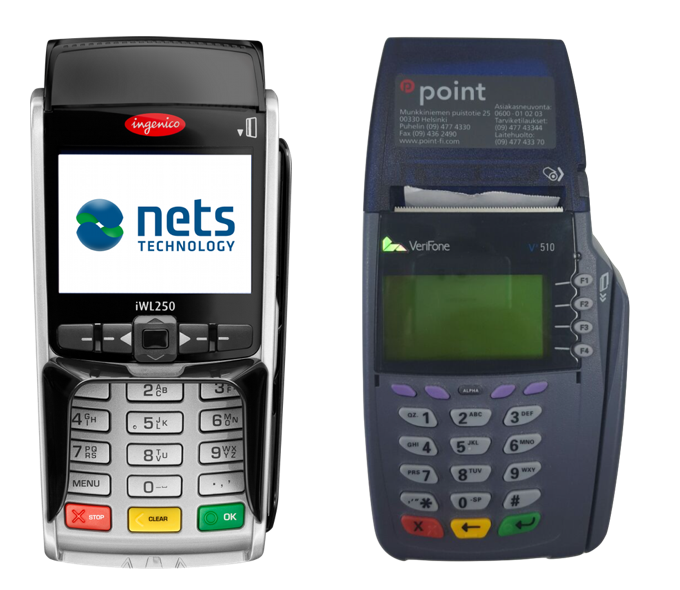
\includegraphics[width=8cm]{images/terminal1.png}
    \caption{Two examples of payment terminals from different manufacturers. Left image from: \url{http://www.netskauppa.fi/images/t/24-85-PrimaryImage.image.ashx}}
    \label{fig:terminals}
  \end{center}
\end{figure}

\begin{figure}[ht]
  \begin{center}
    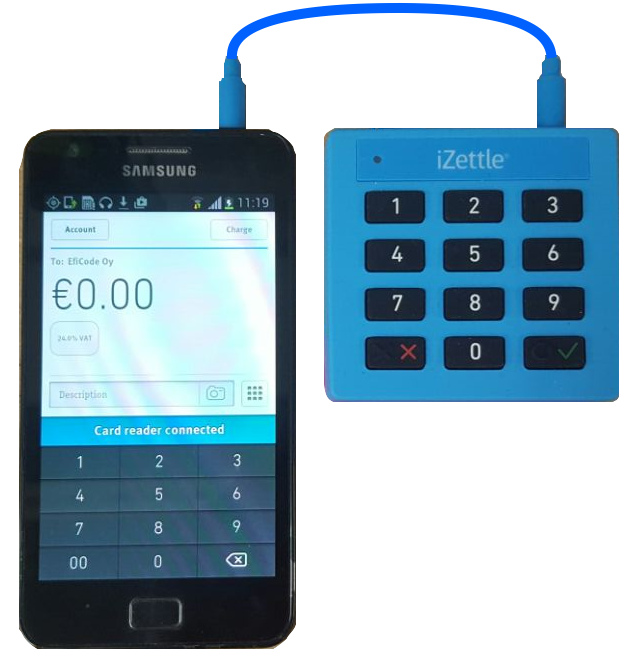
\includegraphics[width=7cm]{images/izettle.png}
    \caption{Example of a payment terminal which attaches to a smart phone.}
    \label{fig:izettle}
  \end{center}
\end{figure}

\section{Different Approaches for Test Automation}
\label{section:test automation approaches}

According to \emph{\cite{broekman2003testing}}, testing of embedded systems and embedded system software can be very different depending on what kind of system is under testing. Mobile phones have to be tested in a very different manner than for example cruise control system in cars. Nevertheless, some general guidelines and divisions exists and should be followed.

Problem of testing a payment terminal software in an automated way can be viewed at different levels. Most abstract division can be seen if the testing is divided into two levels: white box testing and black box testing. White box testing is a method where the source code is investigated and test cases are written to test the internal logic of the program. Black box testing, on the other hand, concentrates only on the inputs and the outputs of the software. Everything between those is not in the field of interest as black box testing only focuses on whether the right input produces the wanted output. (\emph{\cite{myers2011art}})

\emph{\cite{khan2012comparative}} distinguishes these methods clearly from each other by stating that white box testing is a process where full knowledge of source code is needed in order to write the tests. Black box testing is described in a way that only fundamental aspects of the application has to be known and black box testing has no or only little relevance to internal works of the program \emph{\citep{pressman2005software}}. Black box testing techniques can be thus seen to apply for testing of working product against the initial requirements of the software. In this way white box testing can be distinguished to cover unit and integration testing part of the software testing and the black box testing can be seen covering the acceptance testing part of the testing.

As black box testing is based on the external exceptions and behavior of the software \emph{\citep{khan2012comparative}}, acceptance testing of the payment terminal software can be seen to follow this methodology. Intended automated testing of the payment terminals seems to also follow the acceptance testing phase of the division made by \emph{\cite{khan2012comparative}}.

\emph{\cite{huizinga2007automated}}, on the other hand, presents that test automation can be divided into several other layers that are unit testing, integration testing, system testing and acceptance testing. Unit testing is defined to cover testing of a single unit of the software's source code e.g. individual methods and functions of the software. Integration testing is described as a testing phase to verify that different parts of the software work together as a group. System testing is described as being a testing phase where hardware and software is integrated and tested to meet the requirements of the system. This can however include simulated data. Acceptance testing is represented as highest abstraction level of this division as it ensures that the final product meets its acceptance criteria defined by the customers.

\emph{\cite{Ramler}} divides the general architecture of an embedded system into three parts. In this division the human machine interface (HMI) is the top layer. This is followed by the software running on the device and the lowest level are the hardware components of the machine which can be accessed through different analog and digital interfaces. As this master's thesis addresses only the acceptance testing of one instance of an embedded system and as it only has to verify whether the system fulfills its acceptance testing requirements, these abstraction levels can be overlooked. Also for this purpose the black box testing technique seems to be the appropriate testing manner.

Acceptance testing of a payment terminal software can be seen as a testing phase where the UI of the device and the use cases of the device are tested at the final production level, i.e. through using the real buttons of the device under test and observing that the expected messages can be seen through the screen of the same device. This can be seen as an effort to automate a real human user using the payment terminal.

\section{Test Suite Syntax}
\label{section:test suite syntax}

Test suite syntax plays a significant role in an automated acceptance testing environment of payment terminals in terms of test readability, reusability and adaptivity. When building an automated acceptance testing environment, the tests should be understandable enough that the whole development team and all of the project's stakeholders can easily adopt to the test syntax.

According to the well recognized guidelines of test automation by \emph{\cite{snakeoil}}, test automation and the process that it automates should be kept carefully separated. Test automation should be built in a form that it is easy to review and distinct from the process that it automates. These guidelines should be taken into account also when determining a suitable test framework and test suite syntax.

When evaluating suitable test automation frameworks, it should be recognized that shared knowledge is a key factor of successful test automation. Software projects usually involve some sort of quality assurance (QA) or even a separated QA team. Projects also tend to involve fair amount of people with no technical background or coding skills and yet their responsibilities can still involve guaranteeing the quality of the software. \emph{\cite{just_enough}} recognizes that high level test languages help to share the knowledge amongst the people that are responsible for the product. Sharing information and knowledge amongst the project's stakeholders helps achieving the objectives of test automation and builds up the morale amongst the people that are involved.

\emph{\cite{lowell2003successful}} state that acceptance tests should be easy as possible to write or otherwise people working with the project will not write the tests as the task is seen unpleasant. In order to cope with changing requirements or updated features, the tests should be easy to maintain as people have to be able to update them even if they have been written by someone else. For this reason the test cases should be human readable and understandable also to non-technical people. Test steps should be self explanatory and unambiguous.

Test cases in acceptance testing of a payment terminal contain relatively high amount of repetition as for example test step of inserting a personal identification number (PIN) code is the same whether right or wrong PIN code is inserted or whether the test case would validate a credit or debit payment. For this reason, test case syntax should be as modular as possible in order to allow reuse of keywords with different parameters. Easily reusable keywords also allows fast creation of new test cases.

Tests can essentially be written in some conventional coding language, for example Java or Python, or by using some higher level language. There are many widely used test frameworks available for conventional coding languages, for example jUnit for Java \emph{\citep{junit}}. This, however, requires coding experience to some extent in order to be able to understand and modify existing tests or write new ones. As it is stated above, combined with the guideline for writing tests understandable enough, usage of conventional coding languages can be seen opposing the best practices. On the other hand, test case syntax must be versatile enough to accommodate different kinds of testing scenarios and needs. This leads to a situation where the abstraction level of the test cases has to be considered carefully.

\begin{figure}[ht]
  \begin{center}
    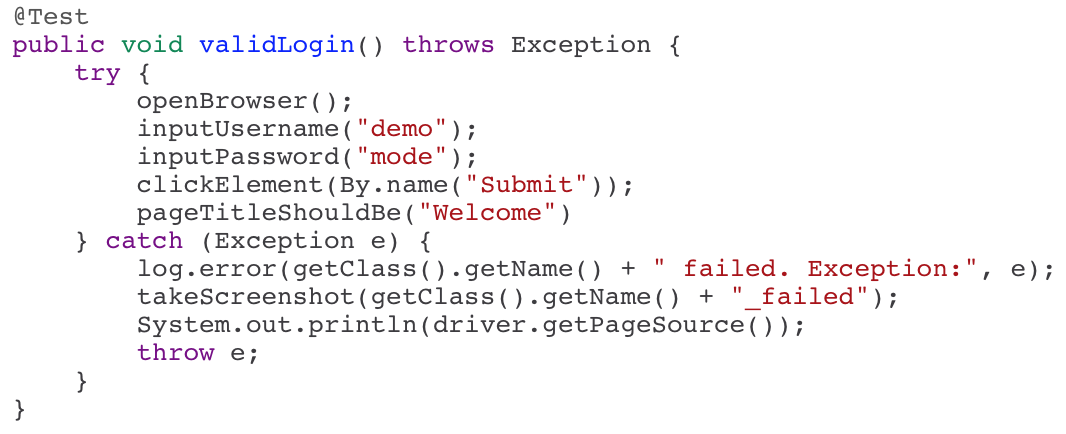
\includegraphics[width=13cm]{images/junit_example.png}
    \caption{Example of a jUnit test case that tries to login to website.}
    \label{fig:junit}
  \end{center}
\end{figure}
\FloatBarrier

In addition to the test frameworks utilizing the use of some conventional coding language for test cases, there are also couple of well recognized tests frameworks available that use a more human-like language for writing the tests. These frameworks usually use the same libraries for interacting with the system under test (SUT) as more low level frameworks but they allow a higher level syntax in the actual test scripts. One fairly popular example of this kind of higher level test framework is Cucumber. Cucumber is an open source acceptance test framework that utilizes behavior-driven development (BDD) style \emph{\citep{cucumber}}. Cucumber uses Gherkin language that is designed to be human readable without previous knowledge of coding \emph{\citep{gherkin}}. This means that also business oriented people involved with the project can understand the test cases.

\begin{figure}[ht]
  \begin{center}
    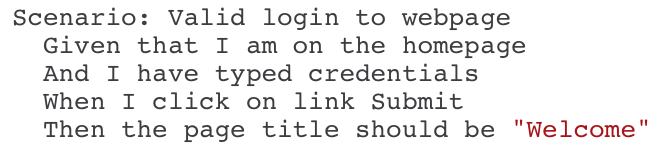
\includegraphics[width=8cm]{images/cucumber_example.png}
    \caption{Example of a simple Cucumber test scenario and use of Gherkin language.}
    \label{fig:cucumber}
  \end{center}
\end{figure}
\FloatBarrier

Another good example of a higher level test framework is Robot Framework (RF). RF is an example of generic keyword driven test automation framework \emph{\citep{robotframework}}. RF allows creation of human readable test cases and reusability and extendibility of high-level keywords is made relatively easy \emph{\citep{stresnjak2011usage}}. \emph{\cite{Rfuserguide}} also outlines that RF has a highly modular software architecture allowing it to be easily connected to any kind of SUT by using different test libraries.

Example of a Robot Framework test case can be seen in Figure~\ref{fig:robot_example} below. It is easy to see the intended test case execution by looking at the test case. This will be the goal for the environment proposed later on in this master's thesis.

\begin{figure}[ht]
  \begin{center}
    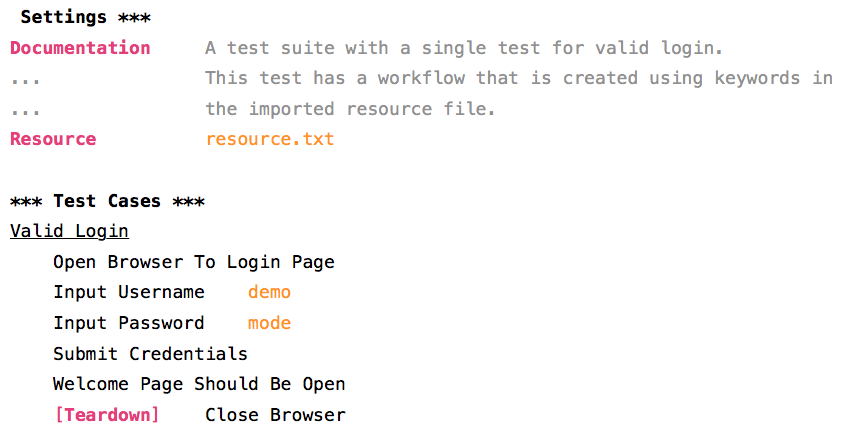
\includegraphics[width=12cm]{images/robot_example.png}
    \caption{Example of a simple test suite. Source: \url{http://robotframework.org}}
    \label{fig:robot_example}
  \end{center}
\end{figure}
\FloatBarrier


%!TEX root = thesis.tex

\chapter{Proposed architecture}
\label{chapter:Proposed architecture}

Based on the aspects pointed out on Chapter~\ref{chapter:Payment terminal acceptance testing}, this part of the master's thesis will present a proposed architecture for automated acceptance testing environment for payment terminal software. Components of the environment can be divided into hardware and software components and this chapter is divided accordingly.

Research done in this master's thesis was carried out in co-operation with Eficode Oy and one of its customers providing payment terminal software in the Nordic countries. Motivation for this project came from the customer and Eficode Oy took responsibility of implementing the system according to the best practices of the industry. This proposal was initial plan for the project and it will be presented in this chapter.

\section{Overview}

When planning an automated acceptance test (AAC) environment for payment terminal software, environment has to be highly adaptive for different types of hardware and software features of different payment terminal models. This proposal was done for one payment terminal software provider and they had several different models of payment terminals and altogether 51 different software configurations for those devices.

Security is a top priority of payment terminal electronics and software and it is not possible to access internals of the payment terminal hardware. This means that AAC environment has to be able to manipulate the physical interface of the device. This also creates requirement for supporting different types of keyboard layouts and screen locations. In other words, environment has to be non dependent on single manufacturer or payment terminal model.

One of the requirements for the AAC environment was also use of open source technologies. For the reasons pointed out in Section~\ref{section:Open source}, customer wanted that the environment is as open as possible. This also creates reputation and visibility regarding the security matters.

Other requirements for the AAC environment was simplicity, low cost, low need for maintenance and ability to run the tests 24/7.

\section{Hardware}
\label{section:Proposed hardware}

Hardware for this proposal was intendedly kept simple and low-cost as possible. This proposal presents the use of just one Raspberry Pi 2\footnote{\url{https://www.raspberrypi.org/products/raspberry-pi-2-model-b/}} computer as a main computer for AAC environment. Raspberry Pi 2 in relatively inexpensive compared to its computing power and it can also run full Linux operating system. It is small sized and does not require any cooling equipment. Therefore it suites well to this project as it can be situated easily to the environment and can be run over the clock without concerns about wearing cooling fans for example.

AAC environment also requires computer vision as changes on the screen have to observed. Manufacturer of Raspberry Pi offers low-price solution for this as a form of Raspberry Pi Camera Module\footnote{\url{https://www.raspberrypi.org/products/camera-module/}}. This module is proposed for use in computer vision tasks of the AAC environment.

\FloatBarrier
\subsection{The Robot}
\label{subsection:The Robot proposal}

To be able to manipulate the physical UI of the payment terminals, some sort of robot is needed. Robot should be therefore able to accommodate different types of payment terminals and be able to press all types of buttons in question. Low cost and low need for maintenance are also requirements for this robot. Robot should also be able to accomodate multiple payment terminals to the working area at the same time in order to allow parrallel execution of acceptance tests. This is intended to speed up the overall process as the same tests have to be run on different models of payment terminals. Other option would also be to make changing of the device under test easy and fast so that the manual work required can be minimized.

The master's thesis proposes the use of ShapeOko 2\footnote{\url{http://www.shapeoko.com/wiki/index.php/ShapeOko_2}} Computer Numerical Control (CNC) milling machine to be used as a manipulator. Though the machine is intended for milling purposes, it can be turned into a portal robot when milling tool is removed.

ShapeOko 2 is an open-source project and plans of the machine are openly available on their GitHub\footnote{\url{https://github.com/shapeoko/Shapeoko_2}}. This allows easy modifications to the hardware parts of the robot if needed.

ShapeOko 2 is controlled by an Arduino board running a program called GRBL. GRBL is an open source, high performance G-code interpreter and it is used for controlling CNC milling machines in general\footnote{\url{http://www.shapeoko.com/wiki/index.php/Software}}. G-code command are sent from Raspberry Pi 2 to the Arduino on the robot using serial communication.

Robot should be equipped with a pushing tool that can be manipulate the buttons. Pushing tool can be easily manufactured using for example 3D printing techniques.

\FloatBarrier
\subsection{Card Feeder}
\label{subsection:Card feeder}

Insertion and removal of the credit card might be hard to accomplish in a simple way using just the robot described in previous section. This work proposes the use of generally designed card feeders to accomplish this task. Proposed card feeders consist of 3D printed base plate that attaches to the payment terminal, servo motor and 3D printed tray that attaches to the servo and to the credit card.

Card feeders are designed in a way that they can be used with any types payment terminals that have the card slot at the bottom edge of the device. Standard hobby servos are used as servo motors in order to keep the cost of the setup low.

Arduino board will be used to drive the servos as it can easily provide the needed pulse width modulated (PWM) signal for the servos. Arduino is suggested in order to ensure quality and accuracy of the PWM signal compared to what can be produced easily with non real time operating system running on the Raspberry Pi. Raspberry Pi on the machine will communicate with Arduino through serial communication.

\section{Software}

For software part of this AAC environment, Raspbian Wheezy is proposed for operating system. Raspbian is the official supported operating system by the Raspberry Pi Foundation\footnote{\url{https://www.raspberrypi.org/downloads/raspbian/}}. Raspbian is based on widely used Debian Unix-like operating system. This allows the use of components developed for Debian to be used with this AAC environment.

As different keyboard layouts have to be supported, some kind of configuration files are proposed. There should be two types of configuration files: one for device locations in the working area of the robot and one for each keyboard layout. In this way configuration of devices under test can be easily modified at test case level.

\FloatBarrier
\subsection{Test Framework}

Robot Framework\footnote{\url{http://robotframework.org/}} is proposed for the test framework. RF is an open-source, generic, keyword-driven test automation framework that has human readable test case syntax (\emph{\cite{Rfuserguide}}).

Robot Framework also has highly modular software architecture (\emph{\cite{Rfuserguide}}) and this allows the framework to be used with any kinds of testing libraries to connect to the system under test. This feature can be seen as a great advantage when implementing test libraries for machine control and computer vision (Chapter~\ref{subsection:test libraries}). Illustration of this modular architecture can be seen in Figure~\ref{fig:modular_architecture} bellow.

\begin{figure}[ht]
  \begin{center}
    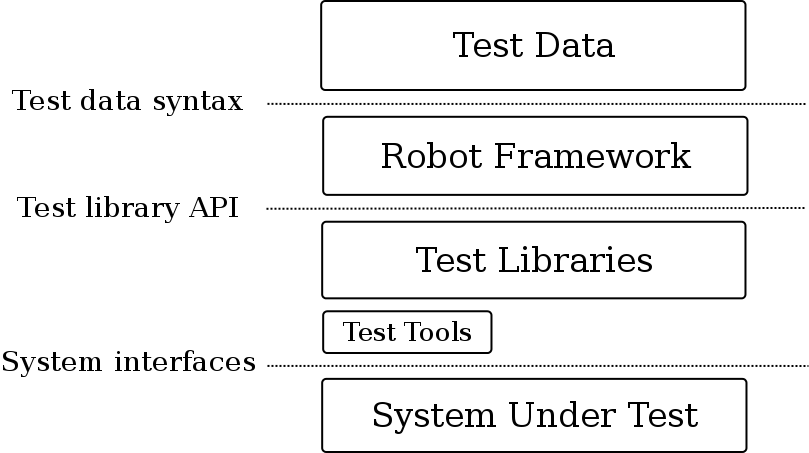
\includegraphics[width=8cm]{images/architecture-big.png}
    \caption{High level modular architecture. Source: \url{http://robotframework.org/img/architecture-big.png}}
    \label{fig:modular_architecture}
  \end{center}
\end{figure}

When RF tests are being run, it generates clear report and log files of the test case execution results (\emph{\cite{Rfuserguide}}). These files offer high level view of all test cases and step-by-step descriptions of individual test cases in order to make the debugging more easy.

Example of intended test case can be seen in Figure~\ref{fig:invalid_pin_test}. This test case describes automated RF acceptance test for entering invalid PIN code when trying to execute card purchase.

\begin{figure}[ht]
  \begin{center}
    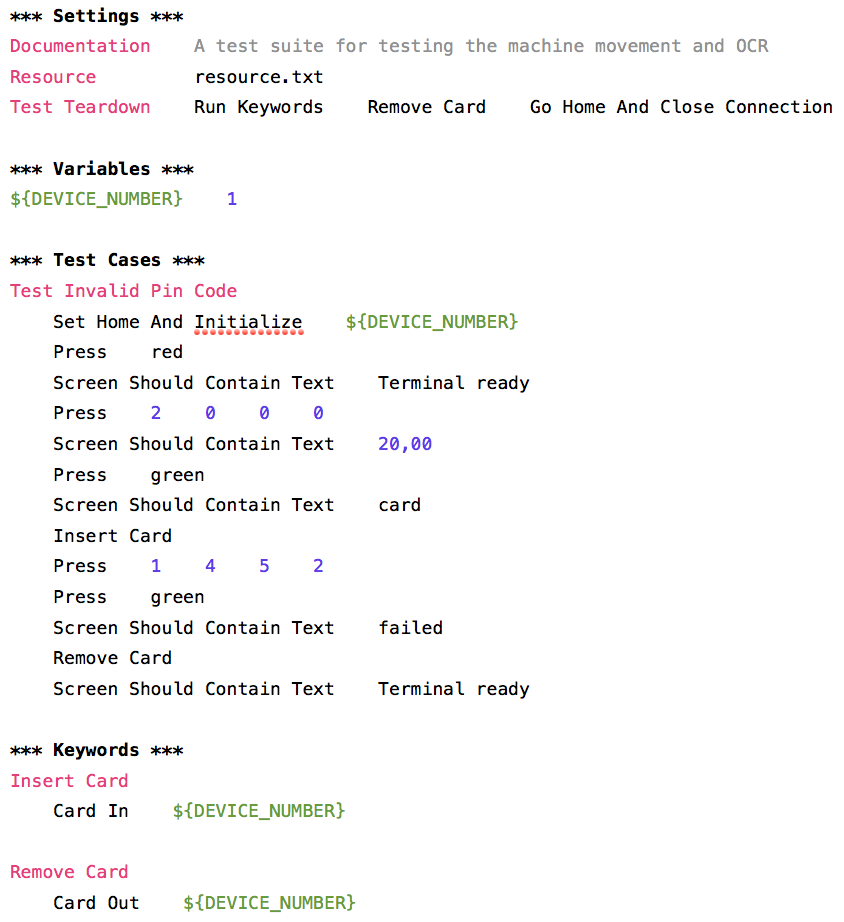
\includegraphics[width=10cm]{images/example_test.png}
    \caption{Example test case for invalid PIN code test}
    \label{fig:invalid_pin_test}
  \end{center}
\end{figure}

\FloatBarrier
\subsection{Test Libraries}
\label{subsection:test libraries}

As can be seen on Figure~\ref{fig:modular_architecture}, architecture requires external libraries to connect to the system under test. In this case those libraries would be a library for machine control, a library for computer vision and a library for card feeder manipulation. All these libraries can be written using Python programming language that is supported out of the box by Robot Framework (\emph{\cite{robotframework}}).

For machine control library the environment has to be able to send G-code command through USB serial communication to Arduino on the robot. For this pySerial\footnote{\url{http://pythonhosted.org/pyserial/}} library is proposed.

For the computer vision task of the environment, messages on the display are usually those that need to be verified. For this character recognition is needed. Open source optical character recognition (OCR) engine called Tesseract OCR\footnote{\url{https://github.com/tesseract-ocr/tesseract}} is proposed. It was initially developed by HP but since 2006 it has been developed by Google. In order to use Tesseract OCR with Python, pytesseract\footnote{\url{https://pypi.python.org/pypi/pytesseract}} wrapper is needed.

Library for controlling the card feeders is the most simplest one of these three libraries. For this pySerial\footnote{\url{http://pythonhosted.org/pyserial/}} library is proposed to send the serial communication command to the Arduino controlling the card feeders.

%%!TEX root = thesis.tex

\chapter{Methods}
\label{chapter:methods}

You have now stated your problem, and you are ready to do something
about it!  \emph{How} are you going to do that? What methods do you
use?  You also need to review existing literature to justify your
choices, meaning that why you have chosen the method to be applied in
your work.

% An example of a traditional LaTeX table
% ------------------------------------------------------------------
% A note on underfull/overfull table cells and tables:
% ------------------------------------------------------------------
% In professional typography, the width of the text in a page is always a lot
% less than the width of the page. If you are accustomed to the (too wide) text
% areas used in Microsoft Word's standard documents, the width of the text in
% this thesis layout may suprise you. However, text in a book needs wide
% margins. Narrow text is easier to read and looks nicer. Longer lines are 
% hard to read, because the start of the next line is harder to locate when
% moving from line to the next. 
% However, tables that are in the middle of the text often would require a wider
% area. By default, LaTeX will complain if you create too wide tables with
% ``overfull'' error messages, and the table will not be positioned properly
% (not centered). If at all possible, try to make the table narrow enough so
% that it fits to the same space as the text (total width = \textwidth).
% If you do need more space, you can either
% 1) ignore the LaTeX warnings 
% 2) use the textpos-package to manually position the table (read the package
%    documentation)
% 3) if you have the table as a PDF document (of correct size, A4), you can use
%    the pdfpages package to include the page. This overrides the margin
%    settings for this page and LaTeX will not complain.
% ------------------------------------------------------------------
% Another note:
% ------------------------------------------------------------------
% If your table fits to \textwidth, but the cells are so narrow that the text
% in p{..}-formatted cells does not flow nicely (you get underfull warnings 
% because LaTeX tries to justify the text in the cells) you can manually set
% the text to unjustified by using the \raggedright command for each cell 
% that you do not want to be justified (see the example below). \raggedleft 
% is also possible, of course...
% ------------------------------------------------------------------
% If you need to have linefeeds (\\) inside a cell, you must create a new
% paragraph-formatting environment inside the cell. Most common ones are 
% the minipage-environment and the \parbox command (see LaTeX documentation
% for details; or just google for ``LaTeX minipage'' and ``LaTeX parbox'').
\begin{table}
\begin{tabular}{|p{2cm}|p{3.8cm}|p{4.5cm}|p{1.1cm}|} 
% Alignment of sells: l=left, c=center, r=right. 
% If you want wrapping lines, use p{width} exact cell widths.
% If you want vertical lines between columns, write | above between the letters
% Horizontal lines are generated with the \hline command:
\hline % The line on top of the table
\textbf{Code} & \textbf{Name} & \textbf{Methods} & \textbf{Area} \\ 
\hline 
% Place a & between the columns
% In the end of the line, use two backslashes \\ to break the line,
% then place a \hline to make a horizontal line below the row 
T-110.6130 & Systems Engineering for Data Communications
    Software & \raggedright Computer simulations, mathematical modeling,
  experimental research, data analysis, and network service business
  research methods, (agile method) & T-110 \\ 
\hline
\multicolumn{2}{|p{6.25cm}|}{Mat-2.3170 Simulation (here is an example of
 multicolumn for tables)}& Details of how to build simulations & T-110 \\
% The multicolumn command takes the following 3 arguments: 
% the number of cells to merge, the cell formatting for the new cell, and the
% contents of the cell
\hline
S-38.3184 & Network Traffic Measurements and Analysis 
& \raggedright How to measure and analyse network
  traffic & T-110 \\ \hline
\end{tabular} % for really simple tables, you can just use tabular
% You can place the caption either below (like here) or above the table
\caption{Research methodology courses}
% Place the label just after the caption to make the link work
\label{table:courses}
\end{table} % table makes a floating object with a title

If you have not yet done any (real) metholodogical courses (but chosen
introduction courses of different areas that are listed in the
methodological courses list), now is the time to do so or at least
check through material of suitable methodological courses. Good
methodologial courses that consentrates especially to methods are
presented in Table~\ref{table:courses}. Remember to explain the
content of the tables (as with figures). In the table, the last column
gives the research area where the methods are often used. Here we used
table to give an example of tables. Abbreviations and Acronyms is also
a long table. The difference is that longtables can continue to next
page.


 
%%!TEX root = thesis.tex

\chapter{Implementation}
\label{chapter:implementation}

You have now explained how you are going to tackle your problem. 
Go do that now! Come back when the problem is solved!

Now, how did you solve the problem? 
Explain how you implemented your solution, be it a software component, a
custom-made FPGA, a fried jelly bean, or whatever.
Describe the problems you encountered with your implementation work.



%%!TEX root = thesis.tex

\chapter{Evaluation}
\label{chapter:evaluation}

You have done your work, but that's\footnote{By the way, do \emph{not} use
shorthands like this in your text! It is not professional! Always write out all
the words: ``that is''.} not enough. 

You also need to evaluate how well your implementation works.  The
nature of the evaluation depends on your problem, your method, and
your implementation that are all described in the thesis before this
chapter.  If you have created a program for exact-text matching, then
you measure how long it takes for your implementation to search for
different patterns, and compare it against the implementation that was
used before.  If you have designed a process for managing software
projects, you perhaps interview people working with a waterfall-style
management process, have them adapt your management process, and
interview them again after they have worked with your process for some
time. See what's changed.

The important thing is that you can evaluate your success somehow.
Remember that you do not have to succeed in making something spectacular; a
total implementation failure may still give grounds for a very good master's
thesis---if you can analyze what went wrong and what should have been done.

 

 
%%!TEX root = thesis.tex

\chapter{Discussion}
\label{chapter:discussion}

At this point, you will have some insightful thoughts on your implementation
and you may have ideas on what could be done in the future. 
This chapter is a good place to discuss your thesis as a whole and to show your
professor that you have really understood some non-trivial aspects of the
methods you used\ldots


 
%!TEX root = thesis.tex

\chapter{Conclusions}
\label{chapter:conclusions}

This seminar report presented a proposal for automated acceptance testing environment for payment terminal software and addressed the theories and problems related to the topic. Presented AAC environment was joint combination of open source hardware and software and was formed by the requirements of a Eficode Oy's customer.

Literature review of this seminar report addressed the four problem statements introduced in the beginning of this seminar report.

This seminar report also lays a promise of how commonly and inexpensively available components can be used in relatively demanding applications. By combining different open source products, highly adaptive AAC environment could be possibly created for the needs of automated acceptance testing of payment terminal software.


% Load the bibliographic references
% ------------------------------------------------------------------
% You can use several .bib files:
% \bibliography{thesis_sources,ietf_sources}
\bibliography{sources}


% Appendices go here
% ------------------------------------------------------------------
% If you do not have appendices, comment out the following lines

%\appendix
%%!TEX root = thesis.tex

\chapter{First appendix}
\label{chapter:first-appendix}

\begin{figure}[htbp]
\begin{center}
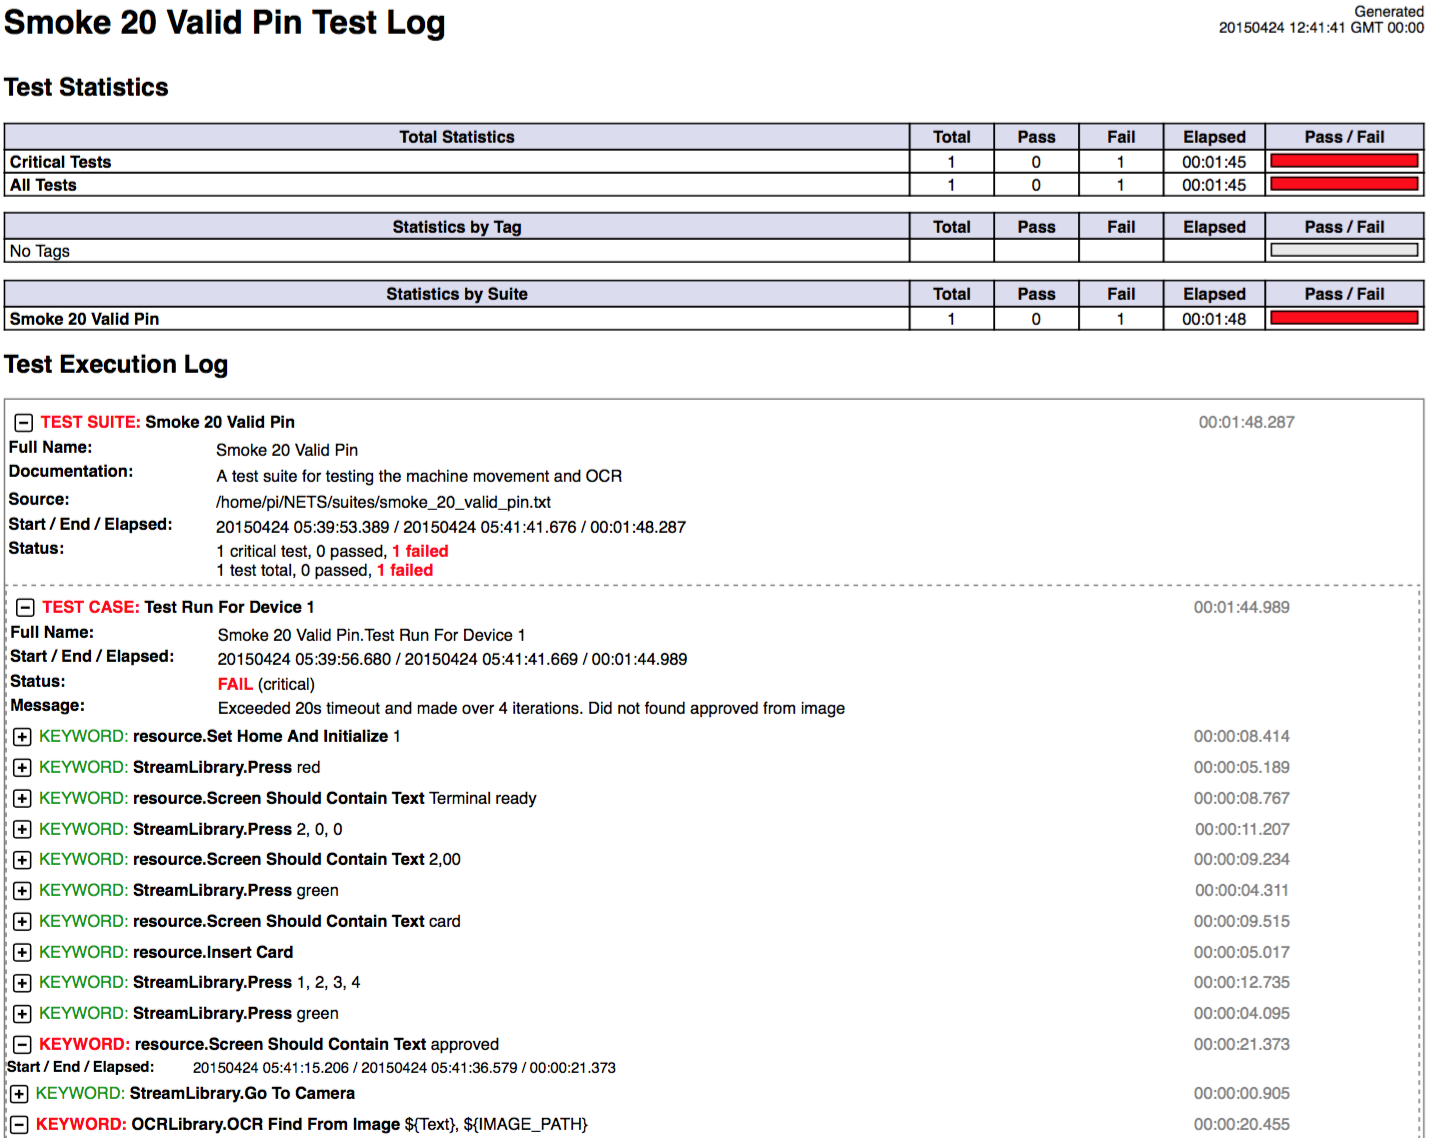
\includegraphics[width=1\textwidth]{images/first_log.png}
\label{fig:passed}
\end{center}
\end{figure}

\begin{figure}[htbp]
\begin{center}
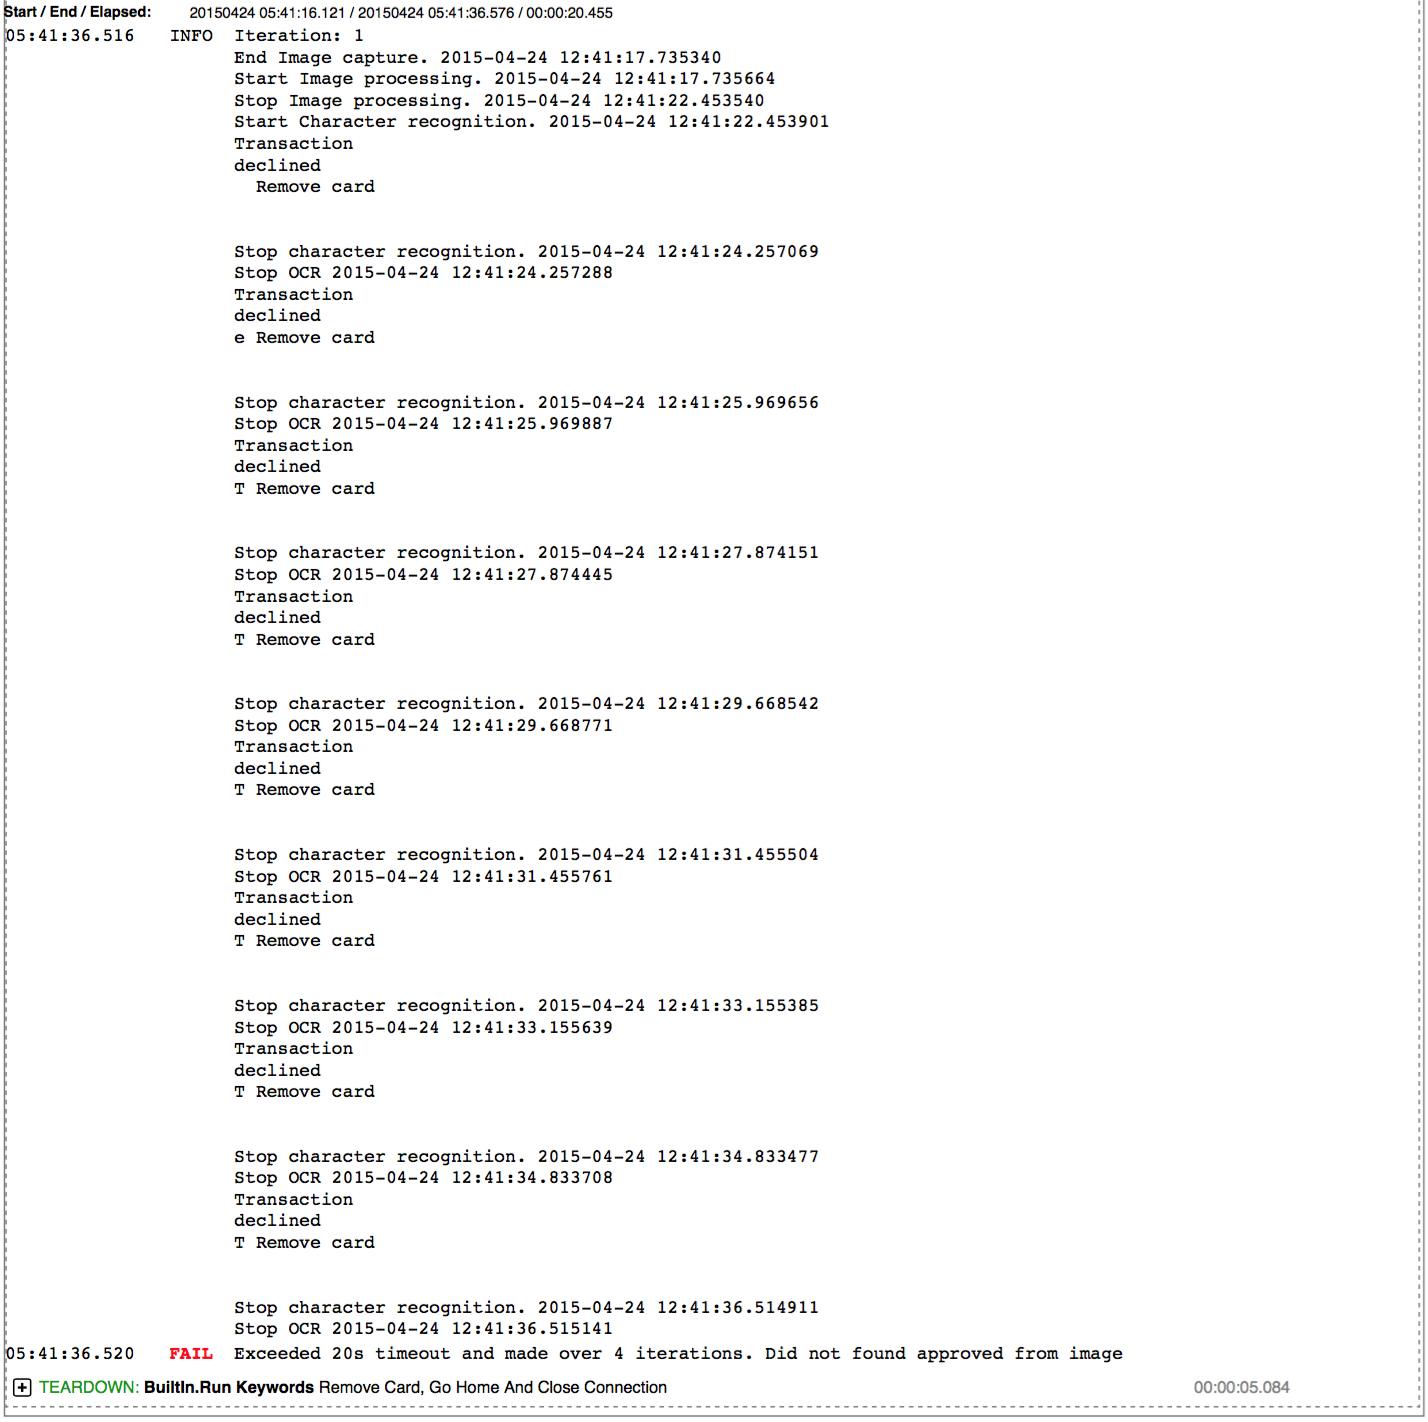
\includegraphics[width=1\textwidth]{images/second_log.png}
\label{fig:passed}
\end{center}
\end{figure}

%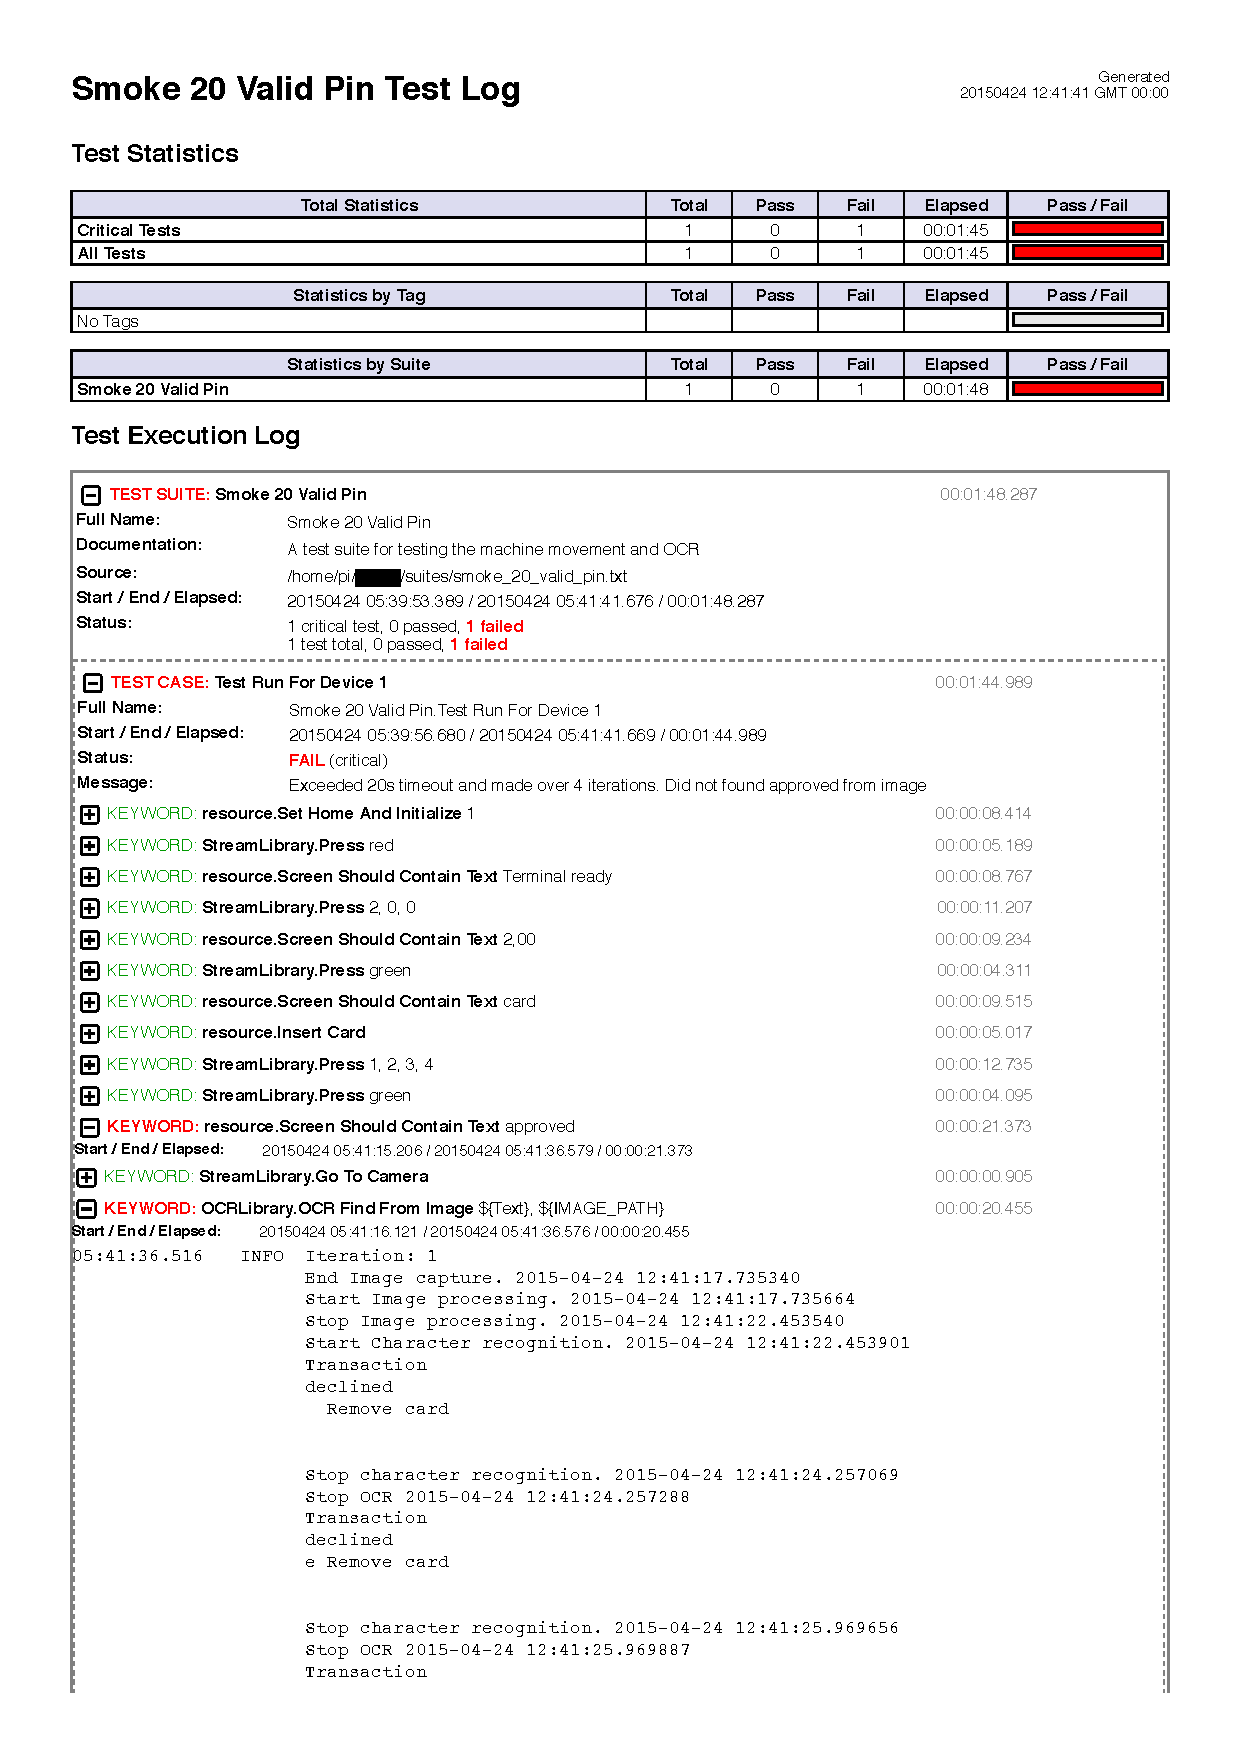
\includepdf[pages=-]{images/smoke_test_log.pdf}

\todos

% End of document!
% ------------------------------------------------------------------
% The LastPage package automatically places a label on the last page.
% That works better than placing a label here manually, because the
% label might not go to the actual last page, if LaTeX needs to place
% floats (that is, figures, tables, and such) to the end of the 
% document.
\end{document}
